
\section{AR Annotation using 3D sensors}
\label{sec:3D}

\begin{figure}[ht]
  \centering
  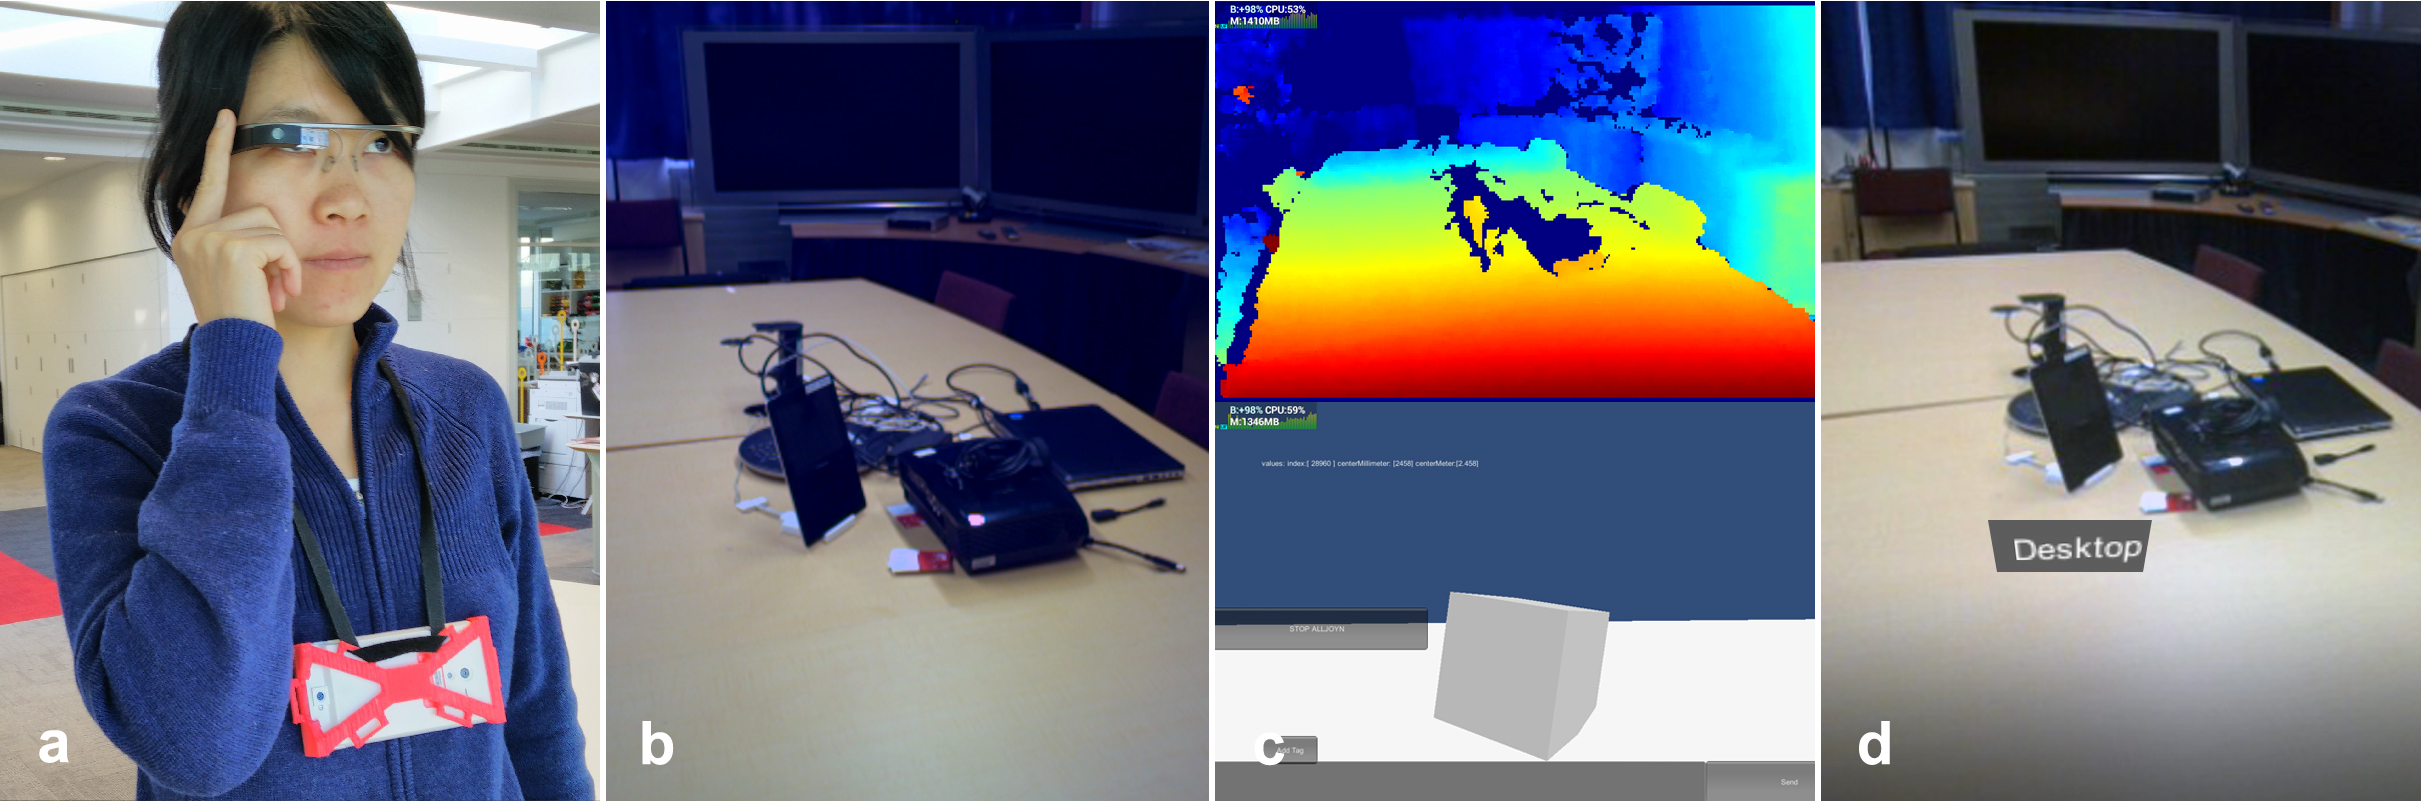
\includegraphics[width=\linewidth]{images/mgia15/sampleteaser-01.jpg}
  \caption{AR annotation application scenario. (a) The user is wearing Google Glass on their head and a Tango device on their chest; (b) A sample indoor environment for spatial tagging; (c) The corresponding depth and visual inertial odometry data from the Tango sensors; (d) The AR view through the Glass display: a virtual tag is now attached to a real location on the table.}
  \label{fig:mgia15:teaser}
\end{figure}

In this work (\cite{Nassani2015a, Nassani2015}, Figure \ref{fig:mgia15:teaser}) we describe a wearable system that allows people to place and interact with 3D virtual tags placed around them. It uses two wearable technologies: a head-worn wearable computer (Google Glass) and a chest-worn depth sensor (Google Tango). The Google Glass is used to generate and display virtual information to the user, while the Tango is used to provide robust indoor position tracking for the Glass. The Tango enables spatial awareness of the surrounding world using various motion sensors including 3D depth sensing, an accelerometer and a motion tracking camera. Using these systems together allows users to create a virtual tag via voice input and then register this tag to a physical object or position in 3D space as an augmented annotation. We describe the design and implementation of the system, user feedback, research implications, and directions for future work.  

This system combines multiple wearable technologies through a wireless network. The system is small and light enough to comfortably wear, allowing for mobility in the physical world, and being available for annotation not only on 2D surfaces but in 3D space. For example, if the user walks closer to or away from the AR tag (e.g., 3D text or models), it will appear larger or smaller according to the changes in the perspective view. The system combines Google Glass and Google Tango together to provide a compelling wearable AR experience. Google Tango is a self-contained handheld device that uses a motion-tracking camera, 3D depth sensing, a nine-axis accelerometer, gyroscope and compass sensors. It has a rear-facing 4MP RGB/infrared camera, a 180-degree field-of-view fisheye rear-facing camera, a 120-degree field-of-view front facing camera, and a 320 x 180 depth sensor. In contrast, Google Glass has no depth sensing capability but combines computing and display in a highly compact form factor. 

% Connecting the two devices enables us to prototype future wearable AR interfaces such as what might be possible with Microsoft Hololens\footnote{https://www.microsoft.com/microsoft-hololens/en-us} or other devices.


\subsection{System Design}

\begin{figure}[ht]
  \centering
  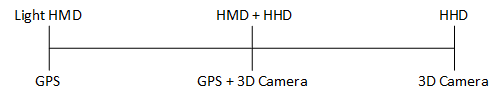
\includegraphics[width=.8\linewidth]{images/mgia15/tango_paper_continuum.png}
  \caption{The spectrum of AR tag tracking. A head-mounted display with GPS is ideal for outdoor tracking. Hand-held devices (3D camera) can be used for indoor tracking. Glass+Tango enables indoor AR tag tracking on a light HMD.}
  \label{fig:mgia15:spectrum}
\end{figure}

The main application scenario for our prototype system is around sharing messages through creating and viewing location-based AR tags registered in a small scale physical environment. The user wearing the system walks into a room and then places AR tags at various places or on objects offline (asynchronously) so that the AR tag can be viewed later by the same user or by a different user. The AR tag content is created by using voice input and placed where the user is looking. The AR tags can be meaningful for users, for example, reminding them of something interesting in this space, or sharing the message with other users as a collaborative tool. The system should work in an arbitrary unprepared indoor environment where no previous knowledge about the space is required. 

Traditionally AR tag tracking uses two different approaches at different ends off the technology spectrum (see Figure\ref{fig:mgia15:spectrum}) based on the level of detailed information required. At one end there is GPS location-based tracking that can be implemented in a light-weight HMD such as Glass. On the other end 3D depth sensing cameras incorporated into a hand-held device (HHD) are capable of indoor tracking and localisation. The aim of this system is to combine the benefits of a light-weight HMD with self-contained mobile 3D depth tracking, offering not only the outdoor GPS based tracking but also vision-based indoor tracking for AR annotation applications. 

\subsection{Implementation}

\begin{figure}
  \centering
  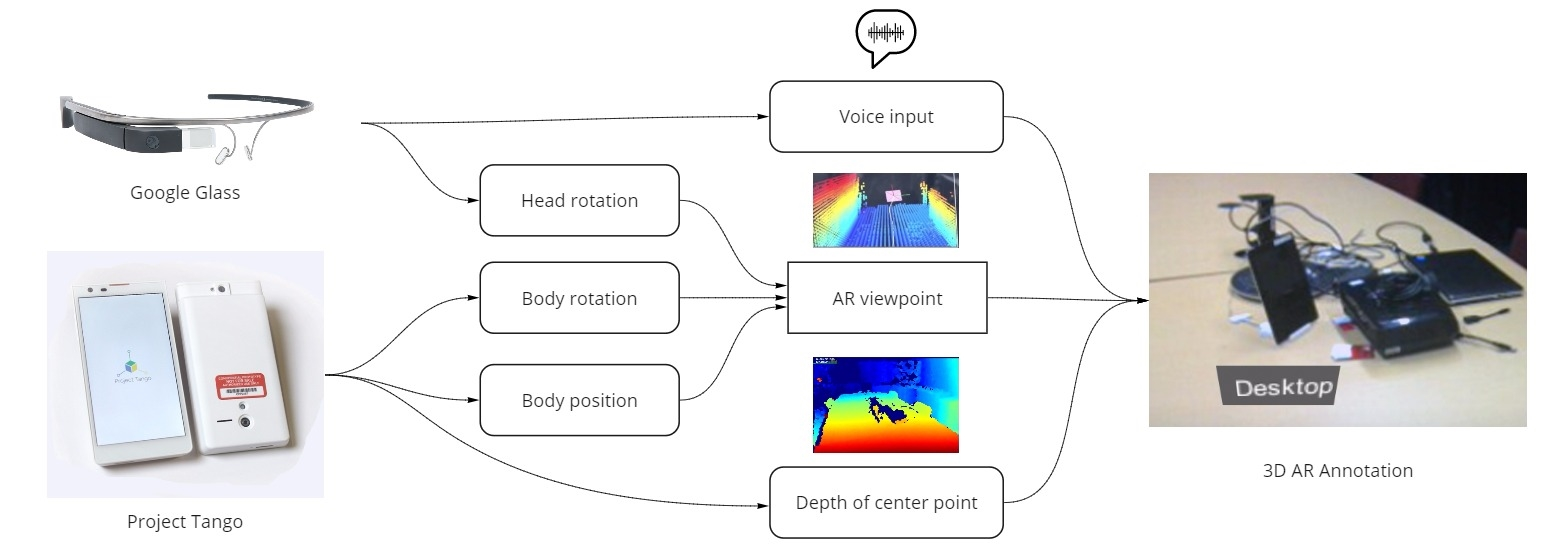
\includegraphics[width=\linewidth]{images/mgia15/mgia2015-system.jpg}
  \caption{System workflow.}
  \label{framework}
\end{figure}

The system consists of two wearable devices, a Google Glass HMD and a Google Tango chest-mounted 3D depth and sensor (see Figure~\ref{framework}). The two devices communicate with each other wirelessly. The Tango extends Glass' sensing ability by sharing the location and pose of the user as well as the tagged target position in the real world. The Glass dynamically overlays virtual tags based on the spatial information received from the Tango, and the background of the Glass display is set to black to act as an optical see through display (see Figure~\ref{fig:mgia15:ui}). A white square is displayed on the Glass screen to indicate the centre point at which the tango depth camera is facing. The user can initiate the wireless connection by using a three-finger touch gesture on the Glass touchpad, and the AllJoyn library  is used for networking.

Once the system starts on the Tango, it creates a reference coordinate of the surrounding environment. When the user moves, the motion sensor on the Tango will detect the body position and rotation from the reference origin, both of which are then wirelessly transmitted to the Glass. Combing the head rotation detected by the sensors on the Glass, we can calculate the AR Viewpoint. The position of the AR viewpoint is calculated by adding a measured distance in height from Tango's position to adjust the height difference between the Glass and Tango. The orientation of the AR viewpoint mainly depends on the body's rotation but will be adjusted with the head and body pose difference, if the user turns their head towards a different direction from their chest. 

\begin{figure}[ht]
  \centering
  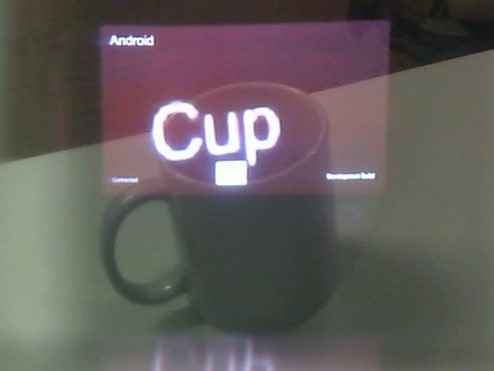
\includegraphics[width=.8\linewidth]{images/mgia15/WIN_20150614_204531_2.jpg}
  \caption{View through Glass display of a cup overlaid with an AR tag.}
  \label{fig:mgia15:ui}
\end{figure}

A speech recognition service is running in the background on the Glass to detect the users' voice input and convert it into text. The text will appear on the upper-left corner of the display for the user's confirmation (see Figure~\ref{fig:mgia15:ui}). The upper-left corner shows the last words captured via the voice recognition service, and a white square indicates the centre position of Tango's RGB depth frame. The text in the middle of the display "Cup" is an AR tag overlaid on top of a physical cup. This function is implemented as an Android service that utilises Google API for speech recognition and so requires an internet connection. Once the user is satisfied with the recognised text, they can tap on the Glass touchpad while looking where they wish to add the AR tag by using the white square in the display. The Glass sends a request to Tango to identify the location of the AR tag in 3D space.

Combining the AR view point and the recognised text, we can convert the target position (the centre point of the depth image indicated by the white square) to the global position relative to the origin. The Tango returns the global position of the AR tag to the Glass. This information is used to construct an AR tag with the speech recognised text that is overlaid on the top of the Glass camera view.

\subsection{User Study}

To evaluate our prototype, we conducted a user study (see Figure~\ref{fig:mgia15:scenario}) with ten participants, four female, six male, ranging in age between 23 to 33 years old ($SD= 4.35$). The main focus of the study was to measure the usefulness of the proposed system. Participants were asked to create three different AR tags for three different objects inside the room, with voice input, and then to walk around to observe how well the AR annotation was placed at the selected location. Participants had the freedom to assign any text to any object they wished in the test. The experimenter explained the tasks before the experiment and gave examples of target objects and names to use for voice input. All participants completed the tasks within five minutes. 

\begin{figure}[ht]
  \centering
  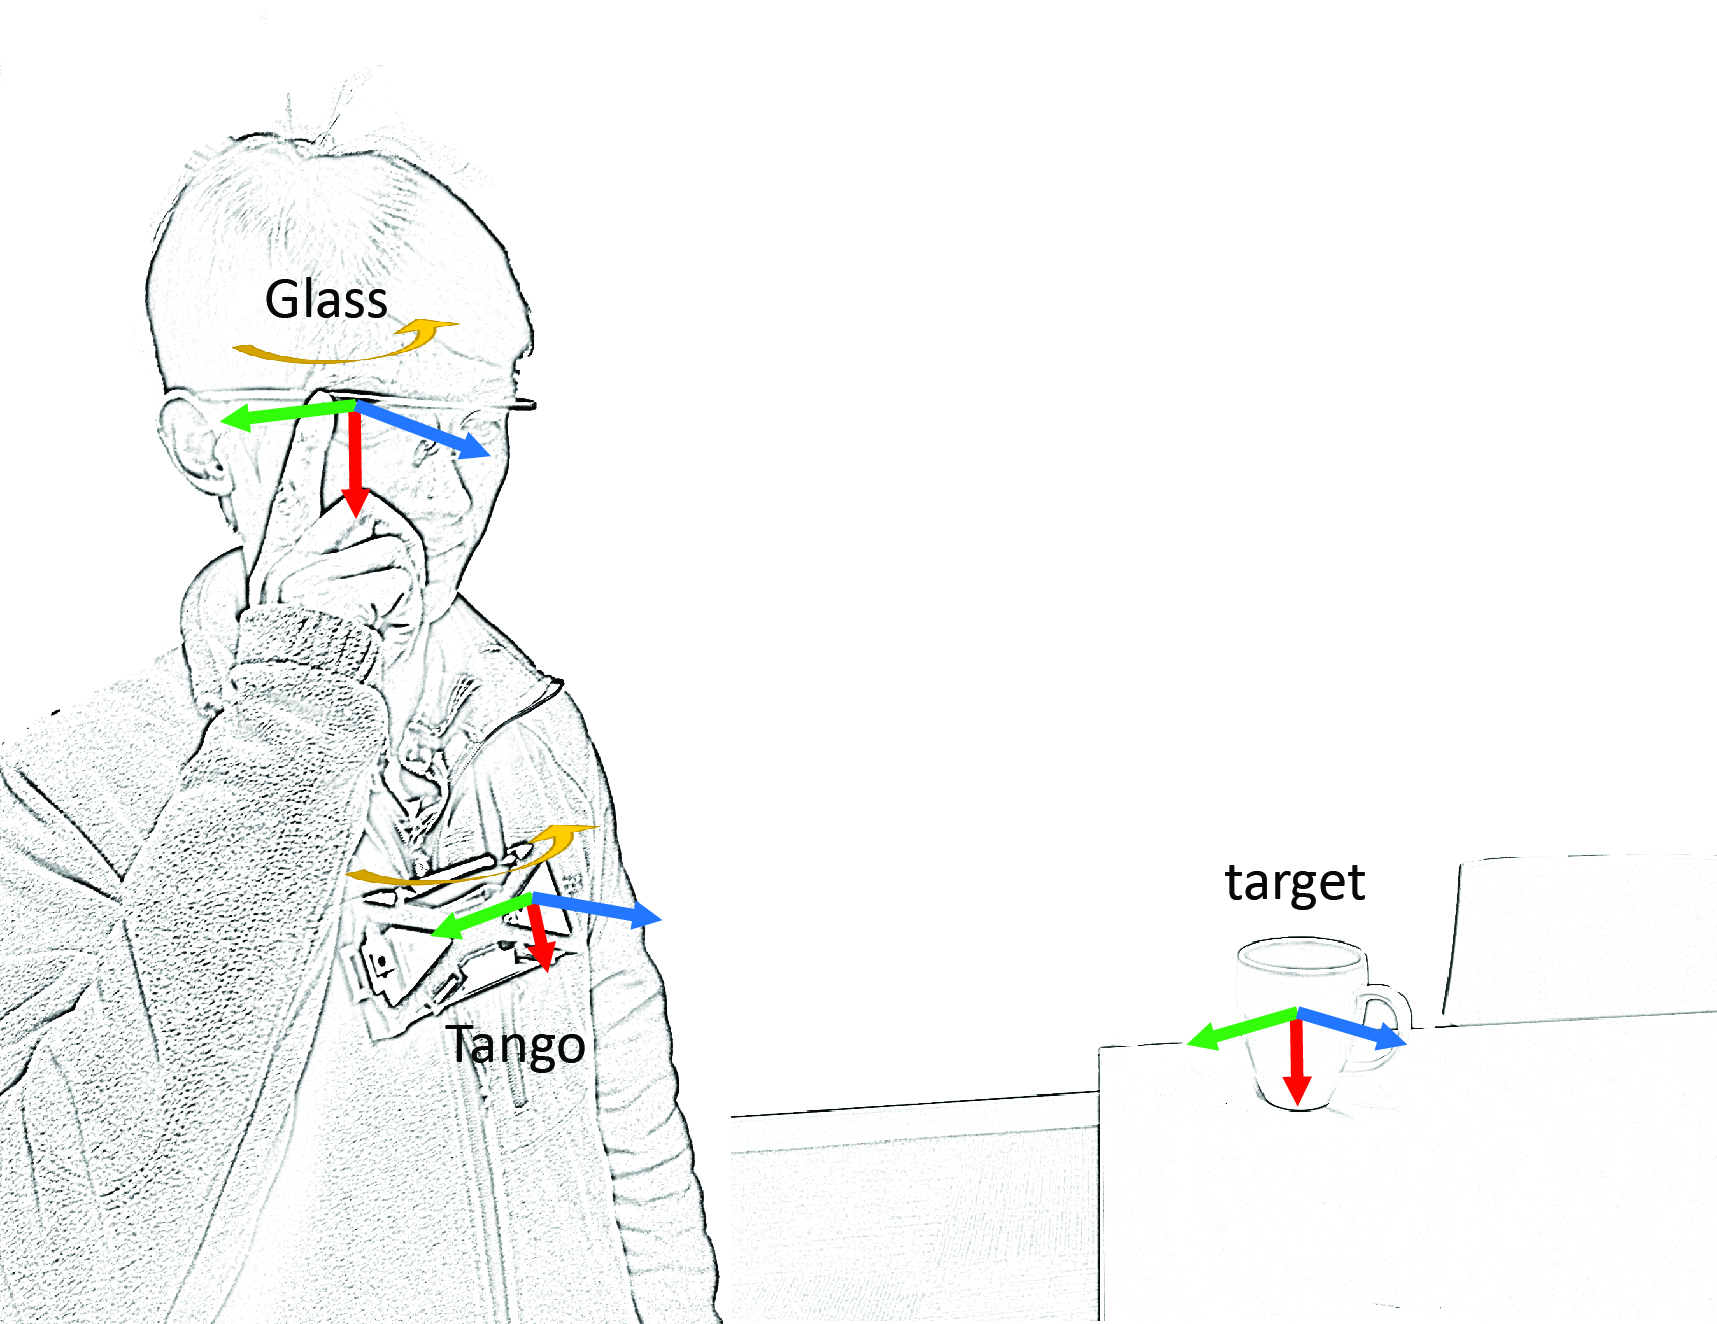
\includegraphics[width=.8\linewidth]{images/mgia15/axis_lo.jpg}
  \caption{User study scenario}
  \label{fig:mgia15:scenario}
\end{figure}

Qualitative feedback about the system was collected from participants including how they would describe their experience using our system, what they liked and disliked. We asked the same set of questions (Table \ref{table:questions}) in four categories: (C1) Using the voice commands to create an AR tag, (C2) Tap on glass touch panel to attach the AR tag, (C3)  Walk around to find an AR tag stuck to the original position, (C4) Overall AR tagging experience.

\begin{table}[ht]
  \centering
	\caption{Survey questions}
    \label{table:questions}
    \begin{tabular}{r l}
    \hline
    Q1 & I found it easy to use \\ \hline
    Q2 & I found it natural to use \\ \hline
    Q3 & I found it physically challenging \\ \hline
    Q4 & I found it mentally challenging \\ \hline
    Q5 & I found it useful \\ \hline
    \end{tabular}
\end{table}

The answers were captured on a Likert scale of 1 to 7 in which 1 was "strongly disagree" and 7 was "strongly agree". We used the Wilcoxon Signed Rank test on the results to measure significance. Based on the results, we found that participants rated significantly higher than neutral (4) on Q3 ($p=0.01, 0.009, 0.007, 0.041$) and Q4 ($p=0.014, 0.009, 0.007, 0.01$) for all categories (C1, C2, C3, C4). Q2 ($p=0.033$) and Q5 ($p=0.015$) were rated significantly higher for category (C3). Q1 for C4 was rated significantly higher ($p=0.014$) (see Figure~\ref{survey_results}). The results  for other tasks were rated less significant than neutral level (4). Participants rated the task of walking around the environment as useful with an average score of 5.2 out of 7, as well as being not mentally challenging with an average score of 2 out of 7. This highlights the usefulness of the system in assigning AR tags and recognising them when they appear on their display while walking around the environment. 

In addition to the survey, we also asked participants open questions to comment on the system usability. A total of 3 out of 5 participants mentioned that they would use this system for virtual sticky notes, and they also provided some positive feedback such as "\textit{the system could be useful for finding a meeting room or a colleague's desk in an open plan area}". There were also a few suggestions for improving the system, such as "allow the user to manually adjust the location of the AR tag" or "integrate with eye tracking to assist placing the AR tag within the field of view ". Participants appreciated  the concept of wirelessly connecting depth camera to a wearable HMD to enable the 3D spatial tracking.    


\begin{figure}[ht]
  \centering
  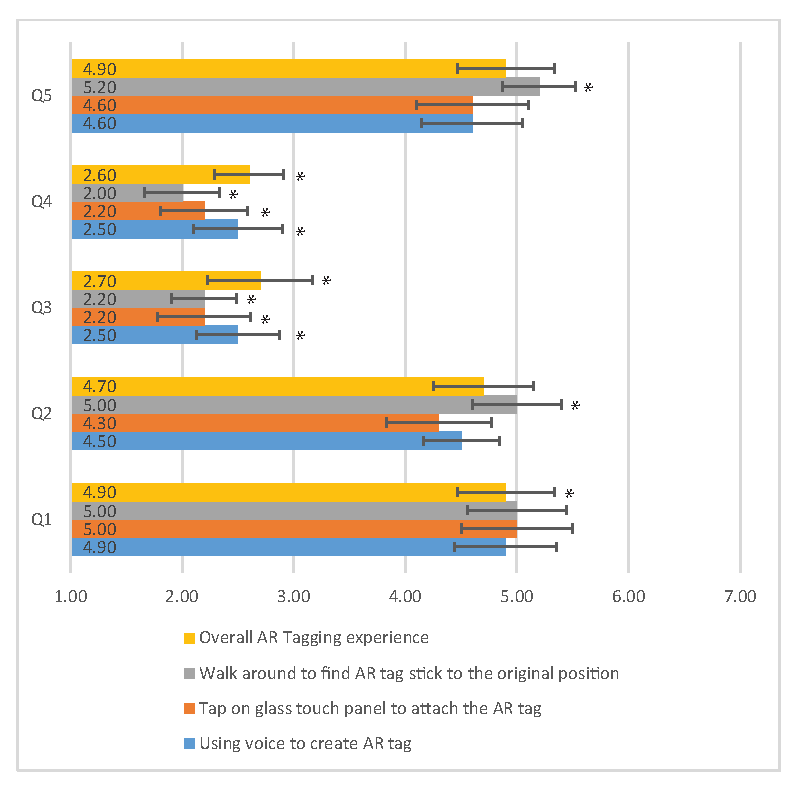
\includegraphics[width=\linewidth]{images/mgia15/user_study_results2.eps}
  \caption{Average results of survey questions. Bars indicate standard error. *=statistically significant}
	\label{survey_results}
\end{figure}


\subsection{Discussion}

While our prototype system demonstrates the concept of harmonising the use of multiple wearable devices for AR visualisation, there are a few limitations in the current implementation of the system. It was observed that some users had difficulties with voice input as they were not native English speakers, which made the participants use several attempts before the intended word was correctly recognised.  

The current system tracks the 3D environment relative to the starting position, which requires users to start the system at the same position and orientation in each test trail to keep the annotation in place between uses for sharing. This could be overcome in the future by storing the reconstructed 3D map of the environment and reusing it instead of generating it from scratch every time. 

\subsection{Future Application Scenarios}

Many implementation scenarios could benefit from combining a light-weight HMD with a chest-worn 3D depth camera, such as 1) Navigation, 2) Remote collaboration and 3) Social sharing. In this section, we describe each of these in more detail.

Navigation is a scenario where this system can be useful. The user could navigate in an outdoor environment using GPS on Glass or similar smart glass display. Google Glass, being an unobtrusive HMD, allows for hands-free navigation. However when the user enters a building, the GPS stops working and the system switches to indoor navigation using the 3D depth camera of the Google Tango device. Combining two devices enables seamless transition during a navigation experience. For example, a person could be shopping to find a particular item and use outdoor GPS tracking to guide them to the store. Once inside the store the Tango depth sensing hardware can help with navigating to find the particular product on the shelf.

Remote collaboration is another scenario where this application could be useful. A local user could transmit reconstructed 3D geometry of the environment using the Tango device to the remote user. The remote user will then have a more detailed view of the environment comparing to 2D sharing such as with a video stream. With the 3D geometry of the environment, the remote user can view the scene from different angles that helps provide better understanding of the surroundings of the local user. Placing AR tags in a 3D environment helps maintain the location of the AR tag especially when the viewing perspective is changed to the point from when it was original recorded

An additional use of the system could be in a social sharing experience where multiple users of the system could collaborate to add, edit and manipulate AR tags in the shared environment. 

\subsection{Summary}

This section presented a wearable AR system combining tracking technologies to provide a compelling indoor AR experience for spatial annotation applications, especially in asynchronous collaboration scenarios where the users of the system are not required to be online at the same time. By wearing the system, users can create virtual tags with text content generated by voice input, and place them where they are looking. The virtual tags can be visualised in place as a reminder for the users.  
